\section{Lösungskonzept} \label{s:solution}
Im folgenden Kapitel werden alle Problematiken aus Kapitel \ref{s:problem} detailliert analysiert und konzeptuelle Lösungsansätze entwickelt.
In Kapitel \ref{ss:cluster-discovery} wird die Integration einer dynamischen HiveMQ Cluster-Discovery in Envoy beschrieben.
Kapitel \ref{ss:load-distribution} untersucht die Lastverteilung in einem HiveMQ Cluster mit Fokus auf die gleichmä{\ss}ige Verteilung von \ac{mqtt} Clients anhand einer Envoy Control-Plane (siehe Kapitel \ref{ss:control-plane}).
Abschlie{\ss}end wird in Kapitel \ref{ss:sticky-session} die Problemstellung der persistenten Client-Sessions (siehe Kapitel \ref{sp:persistent-session}) behandelt.

\subsection{Cluster-Discovery} \label{ss:cluster-discovery}
HiveMQ verfügt über mehrere Mechanismen zur Identifikation von individuellen Nodes, die in das Cluster aufgenommen werden sollen (siehe \ref{s:hivemq-cluster}).
Ein \acl{lb} muss fähig sein, das HiveMQ Cluster auf derselben Datenbasis wie HiveMQ zu formen.
Wenn der \ac{lb} eine andere Datenbasis benutzt, könnte die Topologie des HiveMQ Clusters im \ac{lb} von der tatsächlichen Topologie abweichen.\\
Envoy verfügt über folgende Möglichkeiten, Nodes eines Clusters zu bestimmen:
\begin{itemize}
  \item \textbf{Static:} Alle Nodes eines Clusters werden statisch in die Envoy Konfiguration eingetragen.
  \item \textbf{Strict \ac{dns}:} Envoy löst periodisch und asynchron einen konfigurierten \ac{dns}-Namen auf. Jede eingetragene \ac{ip}-Adresse wird zu einem Node des Clusters. Falls ein Node entfernt wird, werden keine neuen Clients mehr mit diesem Node verbunden. Mit der Variable \verb|dns_refresh_rate| kann die Frequenz, in welcher der \ac{dns}-Eintrag abgefragt wird, bestimmt werden.
  \item \textbf{Logical \ac{dns}:} Ähnlich wie bei Strict \ac{dns} löst Envoy einen konfigurierten \ac{dns}-Namen auf. Bei jeder neuen eingehenden Verbindung wird der \ac{dns}-Name erneut aufgelöst und die erste \ac{ip}-Adresse als Ziel der neuen Verbindung genommen.
  \item \textbf{Original Destination:} Envoy leitet eingehende Verbindungen anhand der \textit{Redirect-Metadata} weiter. Eingehende Verbindungen müssen dafür mit einem \textit{iptables REDIRECT}, \textit{TPROXY target} oder \textit{Proxy-Protocol} an Envoy weitergeleitet werden.
  \item \textbf{Endpoint-Discovery Service:} Envoy ruft die Nodes eines Clusters bei einem \textit{xDS Management-Server} ab. Es werden Java und Golang Bibliotheken angeboten, um einen Management-Server für Envoy zu programmieren und bereitzustellen. Somit ist es möglich, eine komplexe Service-Discovery zu implementieren.
\end{itemize}
\cite{ServiceDiscoveryEnvoy}
In Kapitel \ref{s:hivemq-cluster} wurden folgende Methoden der HiveMQ Cluster-Discovery erläutert:
\begin{itemize}
  \item static
  \item multicast
  \item broadcast
  \item extension
\end{itemize}
Envoy und HiveMQ stellen eine statische Cluster-Discovery zur Verfügung. Diese Methode ist für Cloud- oder Containerumgebungen suboptimal, da sie keine dynamische Veränderung der Cluster-Topologie zulässt. Container-Management-Umgebungen, wie zum Beispiel Kubernetes, erlauben dynamische Vorgänge wie das Skalieren der Replika-Sets oder Rolling-Updates. Eine statische Clusterkonfiguration schlie{\ss}t den Einsatz dieser oder ähnlichen dynamischen Vorgängen aus.\\
Eine weitere gemeinsame Cluster-Discovery Methode ist Strict \ac{dns}. HiveMQ hat diese Methode nicht in der Standardversion implementiert, stellt für diesen Anwendungsfall aber eine frei zugängliche Erweiterung bereit.
Bei Strict \ac{dns} werden periodisch alle Einträge zu einem gegebenen \ac{dns} Eintrag abgefragt und als Nodes des Clusters anerkannt. Die Frequenz der Abfrage wird in Envoy mit der Variable \verb|dns_refresh_rate| bestimmt. In der HiveMQ Erweiterung ist die Einstellung der Frequenz derzeit noch nicht möglich. Ein Issue \cite{AllowConfigurationDiscovery} und ein Pull-Request \cite{ExponentialBackoffGeneral} wurden bereits zu diesem Feature auf GitHub erstellt.
\\
Anders als bei der statischen Clusterkonfiguration ist bei der Strict \ac{dns} Methode eine dynamische Änderung der Nodes möglich. In Cloudumgebungen wie Kubernetes werden \ac{dns}-Zonen dynamisch von Plugins wie \textit{CoreDNS} verwaltet.\cite{DNSServicesPods}
Die Strict \ac{dns} Methode kann auf Änderungen dieser Zonen reagieren und dynamisch die Topologie des HiveMQ Clusters anpassen.
\\
Der Quellcodeauszug \ref{code:envoy-strict-dns} zeigt eine Envoy Clusterkonfiguration, die den \ac{dns}-Namen\newline \verb|example.cluster.internal| auflöst und neue Verbindungen auf alle Einträge an den Port \verb|1883| verteilt.
\begin{figure}
    \import{gen/}{envoy-strict-dns}
    \caption{Es wird eine statische Envoy Cluster Konfiguration gezeigt, die alle Nodes mit der Strict \ac{dns} Methode ermittelt.}
    \label{code:envoy-strict-dns}
\end{figure}
Die \textit{HiveMQ DNS Cluster-Discovery Extension} \cite{HiveMQExtensionDNS} muss auf allen Nodes installiert sein. Der Quellcodeauszug \ref{code:hivemq-dnsdiscovery} zeigt eine Konfigurationsdatei der Erweiterung, die das Cluster aus allen Einträgen des \ac{dns}-Namens \verb|example.cluster.internal| bildet.
\begin{figure}
    \import{gen/}{dnsdiscovery}
    \caption{Dies ist eine HiveMQ \ac{dns} Cluster-Discovery Konfigurationsdatei, die alle 30 Sekunden die Domain \textit{example.cluster.internal} auflöst.}
    \label{code:hivemq-dnsdiscovery}
\end{figure}

\subsection{Lastverteilung HiveMQ Cluster} \label{ss:load-distribution}
In Kapitel \ref{sp:load} wurde erläutert, dass in einem HiveMQ Cluster eine ungleiche Lastverteilung durch die verschiedenen Verhaltensweisen der Clients auftreten kann.
In dem Fall, dass ein Node eine höhere Auslastung als ein anderer Node aufweist, soll die Verteilung neuer Clients an die entstandene Situation angepasst werden.
Es müssen mehr Clients mit Nodes, die eine geringere Auslastung vorweisen, verbunden werden.
Durch den weighted round-robin load balancing Algorithmus wird die Verteilung neuer Clients angepasst. Individuelle Gewichtungen pro Node bestimmen die Wahrscheinlichkeit, mit der ein neuer Client mit einem Node verbunden wird.
\\
Für die Bestimmung der Gewichtungen des weighted round-robin load balancing Algorithmus müssen geeignete Kriterien gefunden werden, die die Auslastungen der einzelnen Nodes widerspiegeln.
Mögliche Indikatoren bieten Systemressourcen wie \ac{cpu}, Arbeitsspeicher, Festplattenspeicher und Netzwerkbandbreite.
Im Rahmen der vorliegenden Arbeit wird untersucht, wie sich ein weighted round-robin load balancing Algorithmus, basierend der \ac{cpu} Auslastungen der einzelnen Nodes, auf den Betrieb des Clusters im Vergleich zu einem round-robin und least-connection load balancing Algorithmus auswirkt.

\subsubsection{Testszenarien} \label{ss:test}
Um den round-robin, least-connection und weighted round-robin load balancing Algorithmus in Bezug auf die gleichmä{\ss}ige Verteilung der Last in einem HiveMQ Cluster zu vergleichen, werden Testszenarien entworfen, die eine ungleiche Lastverteilung in einem HiveMQ Cluster erzeugen.

\begin{itemize}
  \item \textbf{Szenario 1:} In \textit{Bare-Metal} Deployments sind die Server-Kapazitäten an die verfügbare Hardware geknüpft. Es besteht die Möglichkeit, dass ein Cluster aus unterschiedlich dimensionierten Nodes besteht. In Szenario eins besteht das HiveMQ Cluster aus zwei Nodes mit acht \ac{cpu} Kernen und acht \ac{gb} \ac{ram} sowie einem Node mit vier \ac{cpu} Kernen und acht \ac{gb} \ac{ram}. Im Verlauf von zehn Minuten werden sich 5.000 Clients mit ähnlichem Verhalten mit dem Cluster verbinden und Nachrichten veröffentlichen sowie Topics abonnieren.
  \item \textbf{Szenario 2:} Eine dynamische Topologieänderung des HiveMQ Cluster kann durch mehrere Aktionen ausgelöst werden. Dazu zählen Rolling-Upgrades oder Skalierungen des Clusters aufgrund einer Überdimensionierung oder aufgebrauchter Ressourcen. In diesem Szenario wird ein zwei Node Cluster mit jeweils acht \ac{cpu} Kernen und acht \ac{gb} \ac{ram} pro Node mit einem neuen Node mit selben Dimensionen zur Laufzeit erweitert. Vor der Erweiterung sind 3.000 leichtgewichtige Clients mit dem Cluster verbunden. Nach der Erweiterung des Clusters verbinden sich zusätzlich 600 leistungsstarke Clients.
  \item \textbf{Szenario 3:} Die Dimensionen des Clusters sind dieselben wie in Szenario zwei. In diesem Szenario verbinden sich die leistungsstarken Clients vor der Erweiterung und die leichtgewichtigen Clients nach der Erweiterung des Clusters.
\end{itemize}

Szenario zwei wird in folgende Phasen untergliedert:
\begin{itemize}
  \item \textbf{Phase 1:} Formen des Clusters aus zwei Nodes (Node eins und zwei) mit jeweils acht \ac{cpu} Kernen und acht \ac{gb} \ac{ram}.
  \item \textbf{Phase 2:} Verbinden von 3.000 Subscribern, die zufällig 10 von 1.000 Topics abonnieren und jedes Topic mindestens einmal abonniert wird.
  \item \textbf{Phase 3:} Verbinden von 2.000 Publishern. Jeder Publisher veröffentlicht zufällig alle 500 - 2.000 Millisekunden eine Nachricht mit der Payload \verb|Hello World|, einem zufälligen \ac{qos} Level auf ein zufälliges Topic.
  \item \textbf{Phase 4:} Ein dritter Node (Node drei) mit acht \ac{cpu} Kernen und acht \ac{gb} \ac{ram} tritt dem HiveMQ Cluster bei.
  \item \textbf{Phase 5:} Es verbinden sich 300 Publisher. Jeder Publisher veröffentlicht Nachrichten wie in Phase drei beschrieben, jedoch zufällig alle 15 bis 25 Millisekunden.
  \item \textbf{Phase 6:} Es verbinden sich 300 Publisher. Jeder Publisher veröffentlicht Nachrichten wie in Phase vier beschrieben.
\end{itemize}
Szenario drei hat dieselben Phasen wie Szenario zwei in unterschiedlicher Reihenfolge. Phase drei wird mit Phase fünf und sechs getauscht.
\\
Alle Szenarien werden mit einem round-robin und least-connection load balancing Algorithmus ausgeführt, um die Last der einzelnen Nodes zu untersuchen.
Zur Veranschaulichung der Testszenarien werden die \ac{cpu} Auslastungen und deren Standardabweichung mit Grafana visualisiert. Eine blau gestrichelte, senkrechte Linie kennzeichnet das Beenden aller Phasen des jeweiligen Testszenarios. Die Metriken werden alle zwei Sekunden mit Prometheus erfasst.
\\
Die Standardabweichung der \ac{cpu} Auslastungen dient als Indikator für die gleichmä{\ss}ige Verteilung der Last im Cluster. Je kleiner der Wert der Standardabweichung ist, desto gleichmä{\ss}iger ist die Last verteilt.
Die Standardabweichung ist die Quadratwurzel der Varianz und somit ein Ma{\ss} für die Streubreite von Werten um deren Mittelwert in der gleichen Ma{\ss}einheit.\cite[S.~72]{buchterElementareStochastikEinfuhrung2005}. Die Standardabweichung wird mit der Prometheus Funktion \verb|stddev| berechnet.
\newpage

\paragraph{Szenario 1}
Abbildung \ref{fig:s1-rr} und \ref{fig:s1-lc} zeigen den zeitlichen Verlauf von Testszenario eins für einen round-robin und least-connection \acl{lb}.
Beide verhalten sich in diesem Szenario ähnlich. Alle Clients werden gleichmä{\ss}ig auf die Nodes verteilt.
Da die Clients ein ähnliches Verhalten aufweisen, entsteht auf jedem Node eine gleiche Belastung. Node drei hat nur die Hälfte der \ac{cpu} Kerne zur Verfügung wie Node eins und zwei und ist daher nicht in der Lage, die Last so schnell abzuarbeiten wie Node eins oder zwei. Somit entsteht ein ungleiches Lastverhalten im Cluster.
\begin{figure}[h]
    \centering
    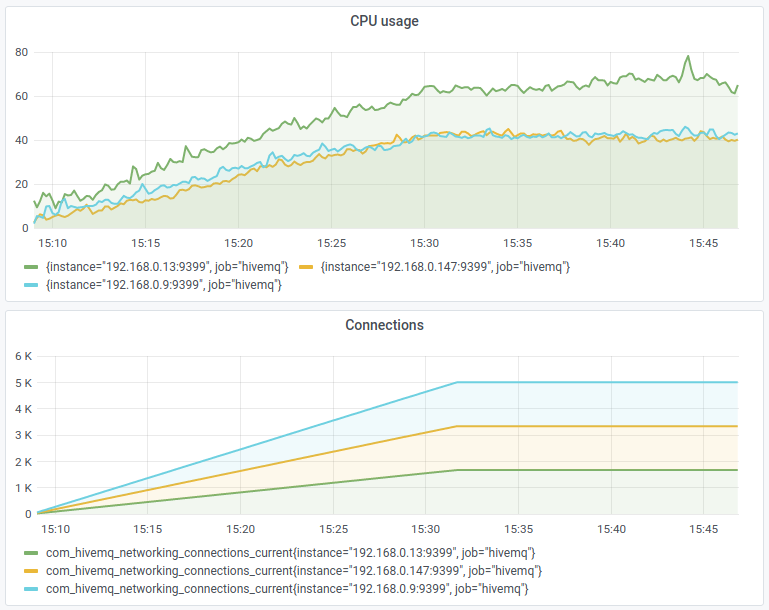
\includegraphics[scale=0.8]{images/s1_lc.png}
    \caption{Testszenario 1 - least-connection \acl{lb}}
    \label{fig:s1-lc}
\end{figure}
\begin{figure}[h]
    \centering
    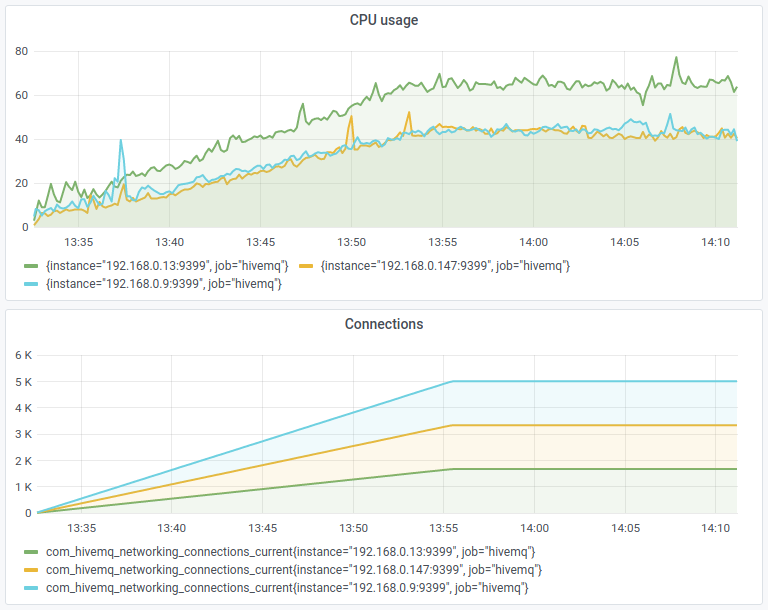
\includegraphics[scale=0.8]{images/s1_rr.png}
    \caption{Testszenario 1 - round-robin \acl{lb}}
    \label{fig:s1-rr}
\end{figure}

\paragraph{Szenario 2 - Least-Connection}
Abbildung \ref{fig:s2-lc} zeigt den zeitlichen Verlauf von Testszenario zwei bei einem least-connection \ac{lb}.
Nach Abschluss von Phase sechs hat dieses Szenario eine Standardabweichung von zehn Prozent.
Die Last auf dem Cluster ist ungleich verteilt, da Node drei doppelt so hoch ausgelastet ist wie Node eins und Node zwei.
Dieses Ungleichgewicht wird durch Phase sechs verstärkt. Auf Node eins und Node zwei sind jeweils 3.500 Clients verbunden auf Node drei hingegen nur 300 Clients. Der least-connection \acl{lb} verteilt nun alle Clients aus Phase sechs auch auf Node drei. Trotz der noch höheren Auslastung auf Node drei würden die nächsten 2.900 Clients ebenfalls mit Node drei verbunden werden.
\newpage
\begin{figure}[h]
    \centering
    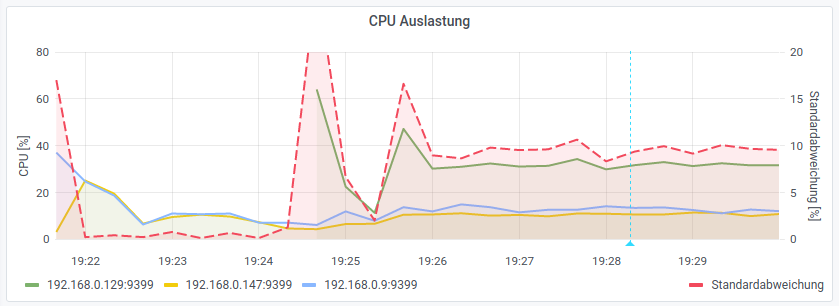
\includegraphics[scale=0.8]{images/s2_lc.png}
    \caption{Testszenario 2 - least-connection \acl{lb}}
    \label{fig:s2-lc}
\end{figure}

\paragraph{Szenario 2 - Round-Robin}
Abbildung \ref{fig:s2-rr} zeigt den zeitlichen Verlauf von Testszenario zwei bei einem round-robin \ac{lb}.
Nach Abschluss von Phase sechs hat dieses Szenario eine Standardabweichung von drei Prozent.
Nach Phase fünf und sechs ist die Last auf dem Cluster im wesentlichen gleichmä{\ss}ig verteilt. Node eins und zwei sind um die Anzahl der Clients aus Phase zwei und drei stärker belastet. Diese sind jedoch leichtgewichtige Clients und erzeugen demnach nicht viel Last auf den Nodes.
Der round-robin Algorithmus verteilt alle Clients gleichmä{\ss}ig auf dem Cluster.
Daher werden nach dem Beitreten von Node drei in Phase vier nicht wie bei dem least-connection Algorithmus alle neuen Clients auf den neuen Node verteilt.
\begin{figure}[h]
    \centering
    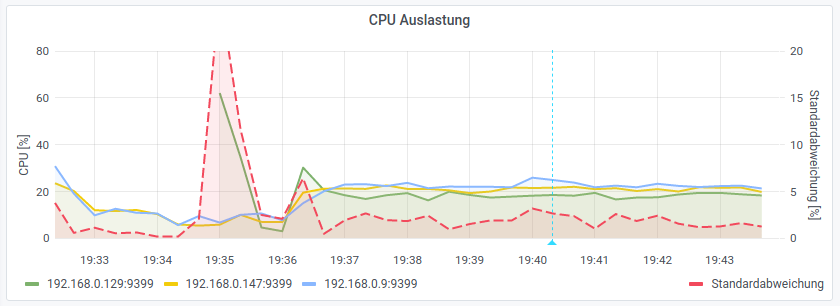
\includegraphics[scale=0.8]{images/s2_rr.png}
    \caption{Testszenario 2 - round-robin \acl{lb}}
    \label{fig:s2-rr}
\end{figure}

\paragraph{Szenario 3 - Least-Connection}
Abbildung \ref{fig:s3-lc} zeigt den zeitlichen Verlauf von Testszenario drei bei einem least-connection \ac{lb}.
Nach Abschluss von Phase sechs hat dieses Szenario einen Lastindikator von sechs.
Node eins und zwei sind mehr belastet als Node drei, da alle Clients aus Phase drei und vier mit diesen beiden Nodes verbunden sind. Alle Clients aus Phase sechs sind mit Node drei verbunden, jedoch verursachen diese nicht so viel Arbeitslast wie die Clients aus Phase drei und vier.
\newpage
\begin{figure}[h]
    \centering
    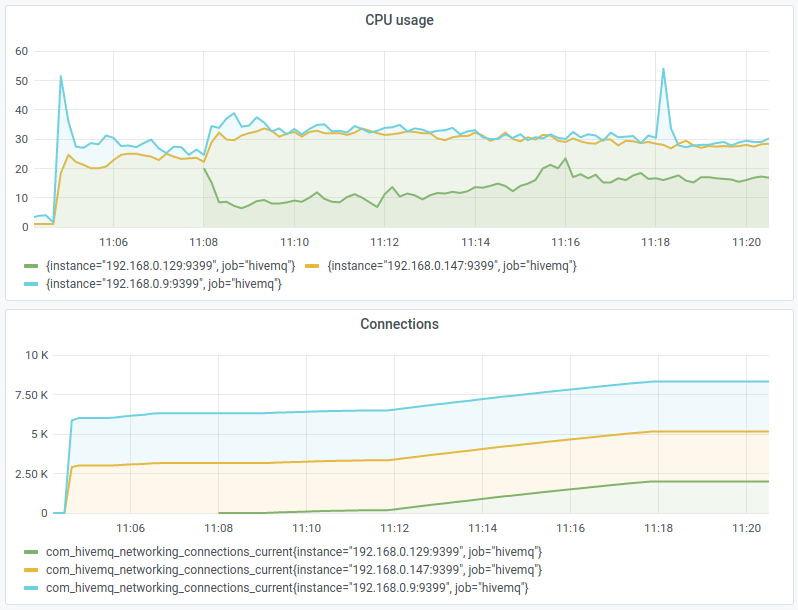
\includegraphics[scale=0.8]{images/s3_lc.png}
    \caption{Testszenario 3 - least-connection \acl{lb}}
    \label{fig:s3-lc}
\end{figure}

\paragraph{Szenario 3 - Round-Robin}
Abbildung \ref{fig:s3-rr} zeigt den zeitlichen Verlauf von Testszenario drei bei einem round-robin \ac{lb}.
Nach Abschluss von Phase sechs hat dieses Szenario eine Standardabweichung von acht Prozent.
Nach Phase sechs sind Node eins und zwei jeweils dreifach so sehr ausgelastet wie Node drei. Die Last auf dem Cluster ist somit ungleich verteilt.
Die Clients aus Phase drei und vier werden nur auf Node eins und zwei verteilt, da der dritte Node noch nicht dem Cluster beigetreten ist. Die leichtgewichtigen Clients aus Phase sechs werden durch den round-robin Algorithmus auf alle Nodes verteilt, obwohl Node drei gar nicht ausgelastet ist. Im Idealfall würde der \ac{lb} alle 3.000 Clients aus Phase sechs auf Node drei verteilen.
\begin{figure}[h]
    \centering
    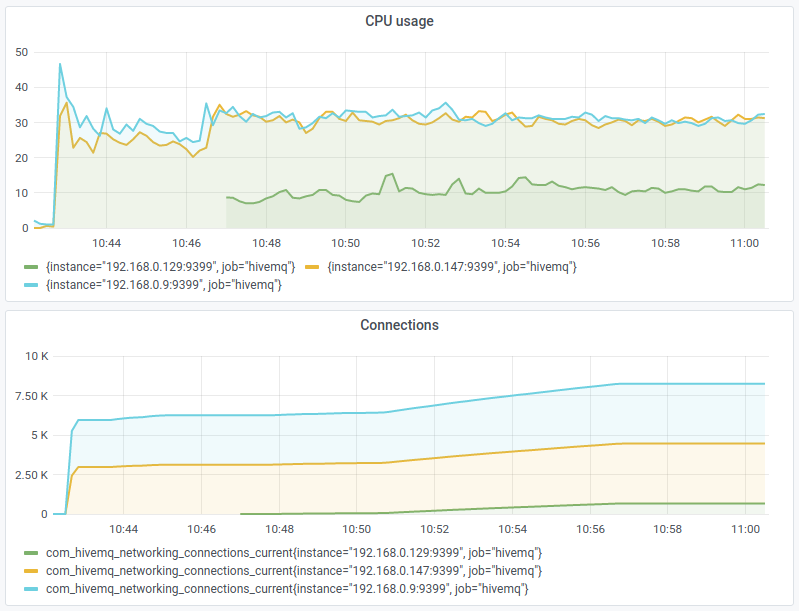
\includegraphics[scale=0.8]{images/s3_rr.png}
    \caption{Testszenario 3 - round-robin \acl{lb}}
    \label{fig:s3-rr}
\end{figure}

\newpage
\subsubsection{Weighted Round-Robin} \label{ss:weighted-rr}
Kapitel \ref{ss:test} zeigt, dass ein least-connection \acl{lb} in Szenario drei und ein round-robin \ac{lb} in Szenario zwei die Last gleichmä{\ss}ig verteilen kann.
Bei den anderen Szenarien befindet sich das Cluster anschlie{\ss}end in einem ungleichen Lastverhältnis.
Da \ac{mqtt} auf langlebigen \ac{tcp}-Verbindungen basiert, wird sich dieses Lastverhältnis nicht verändern, bis die Clients ihre Verbindung neu aufbauen oder ihr Verhalten verändern.
Der \ac{lb} muss dynamisch auf ein bestimmtes Client-Verhalten reagieren und Clients basierend auf der Arbeitslast der einzelnen Nodes verteilen.
\\
Bei dem weighted round-robin load balancing Algorithmus wird jedem Node eines Clusters eine Gewichtung zugeordnet. Die Gewichtung des Nodes bestimmt die Wahrscheinlichkeit, mit der ein neuer Client mit einem Node verbunden wird.
Um mehr Clients mit Nodes von geringerer Auslastung zu verbinden, muss die derzeitige Auslastung direkten Einfluss auf die Gewichtung des Nodes haben.
Diese Mechanik wird bereits bei anderen Protokollen wie \ac{http} eingesetzt.
Eine load balancing Entscheidung bei \ac{mqtt} ist jedoch relevanter als bei Protokollen wie \ac{http}, weil die Entscheidung für die Dauer der Verbindung nicht mehr verändert werden kann. Da \ac{mqtt} von langlebigen \ac{tcp}-Verbindungen profitiert, kann der \ac{lb} die Last eines bestimmten Clients nach dem Verbindungsaufbau nicht mehr steuern.
\\
Envoy hat mehrere load balancing Algorithmen, unter anderem weighted round-robin, implementiert.
Jedem Node eines Clusters wird eine Gewichtung in Form eines Integer-Wertes zugeordnet.
Je grö{\ss}er der Wert im Verhältnis zu allen anderen Nodes des Clusters ist, desto höher ist die Wahrscheinlichkeit, dass ein neuer Client mit dem Node verbunden wird. Der Wert der Gewichtung muss grö{\ss}er als eins und die Werte aller Nodes addiert dürfen nicht grö{\ss}er als 4294967295 sein.
Um den Prozentsatz zu berechnen, wie viele Clients mit einem individuellen Node verbunden werden, teilt Envoy die Gewichtung des jeweiligen Nodes durch die Summe der Gewichtungen aller Nodes und multipliziert das Ergebnis mit 100.
\cite{SupportedLoadBalancers}
\\
Tabelle \ref{table:example-cluster-weight} zeigt drei Nodes mit ihren Gewichtungen und den dazu errechnetem Prozentsatz aller Clients, die mit diesem Node verbunden werden.
\begin{table}[h!]
\centering
\renewcommand{\arraystretch}{1.5}
\begin{tabular}{|l|c|c|}
    \hline
    \textbf{Node} & \textbf{Gewichtung} & \textbf{Prozent Traffic} \\
    \hline
    \hline
    Node 1 & 10 & 40\% \\
    \hline
    Node 2 & 10 & 40\% \\
    \hline
    Node 3 & 5 & 20\% \\
    \hline
\end{tabular}
\caption{Die Tabelle zeigt drei Nodes eines Clusters und ihren Gewichtungen bei einem weighted round-robin load balancing Algorithmus des Envoys. Die Spalte \textit{Prozent Traffic} gibt an, mit welcher Wahrscheinlichkeit ein neuer Client mit diesem Node verbunden wird.}
\label{table:example-cluster-weight}
\end{table}
\\
Der Quellcodeauszug \ref{code:envoy-cluster-weight} zeigt eine statische Envoy Konfiguration, um ein Cluster aus drei Nodes mit den Gewichtungen aus Tabelle \ref{table:example-cluster-weight} zu formen.
\begin{figure}
    \import{gen/}{envoy-weighted-round-robin}
    \caption{Es wird eine statische Envoy Cluster Konfiguration gezeigt, bei der neue Clientverbindungen basierend dem weighted round-robin load balancing Algorithmus verteilt werden.}
    \label{code:envoy-cluster-weight}
\end{figure}
\newpage\noindent
Die Problematik bei der Konfiguration aus Quellcodeauszug \ref{code:envoy-cluster-weight}, ist die statische Angabe der Nodes mit ihren Gewichtungen.
Eine dynamische Cluster-Discovery wie in Kapitel \ref{ss:cluster-discovery} beschrieben, ist nicht möglich.
Neben der statischen Konfigurationsdatei bietet Envoy zwei Mechanismen für eine dynamische Konfiguration an.
\begin{itemize}
  \item \textbf{Dynamisch via Dateisystem:} Envoy liest Konfigurationsdateien, die das xDS Protokoll implementiert haben, vom Dateisystem ein. Wenn sich die Dateien in dem Dateisystem ändern, aktualisiert Envoy automatisch seine Konfiguration.
    \cite{ConfigurationDynamicFilesystem}
  \item \textbf{Dynamisch via Control-Plane:} Envoy bezieht seine Konfiguration dynamisch von einer Control-Plane. Eine Control-Plane ist ein \ac{api} Server, der Konfigurationen an Envoy Instanzen schickt. Die Schnittstelle, um Konfigurationen zwischen Envoy und Control-Plane auszutauschen, ist in der \textit{Data-Plane API} (siehe \cite{EnvoyproxyDataplaneapi2021}) dokumentiert.
    \cite{ConfigurationDynamicControl}
\end{itemize}
Die dynamische Konfiguration via Dateisystem ist geeignet für einzelne Envoy Instanzen, da keine individuelle Control-Plane programmiert werden muss.
Möchte man jedoch mehrere Envoy Instanzen mit derselben Konfiguration betreiben, muss bei einer Aktualisierung der Konfiguration die neue Datei auf die Dateisysteme aller Envoys verteilt werden.
Für den Anwendungsfall mehrerer Envoy Instanzen ist das dynamische Verteilen mit einer Control-Plane besser geeignet. Jeder Envoy wird mit einer statischen Datei konfiguriert, in der die Adresse der Control-Plane eingetragen ist. Sobald eine Envoy Instanz startet, registriert sich diese an der Control-Plane und erhält seine Konfiguration. Das Verteilen von Konfigurationsaktualisierungen an die Envoy Instanzen wird nun von der Control-Plane übernommen.
\\
Quellcodeauszug \ref{code:envoy-control-plane} zeigt eine statische Konfigurationsdatei zur Registrierung bei einer Control-Plane, die unter \verb|example.controlplane.internal:18000| erreichbar ist.
\begin{figure}
    \import{gen/}{envoy-control-plane}
    \caption[Statische Envoy Konfiguration, um eine gRPC-Verbindung mit einer Control-Plane aufzubauen.]{Der Quellcodeauszug zeigt eine statische Envoy Konfiguration, um eine gRPC-Verbindung mit einer Control-Plane unter der Adresse {example.controlplane.internal:18000} aufzubauen.}
    \label{code:envoy-control-plane}
\end{figure}
Die Konfigurationsdatei ist in drei Teile gegliedert:
\begin{itemize}
  \item \verb|node:| Identifikation der Envoy Instanz bei der Control-Plane. Eine Control-Plane kann verschiedene Konfigurationen verwalten. Durch \verb|node.id| kann die Envoy Instanz einer Konfiguration zugeordnet werden.
  \item \verb|dynamic_resources:| Gibt die Quelle der dynamischen Provisionierung an. Im Quellcodeauszug \ref{code:envoy-control-plane} wird eine g\acs{rpc} \ac{api} Namens \verb|xds_cluster| verwendet.
  \item \verb|static_resources:| Es wird die Quelle für eine dynamische Provisionierung definiert. Im Quellcodeauszug \ref{code:envoy-control-plane} wird eine Quelle namens \verb|xds_cluster| definiert. Diese Quelle wird in \verb|dynamic_resources| referenziert.
\end{itemize}
Eine Control-Plane kann in jeder Programmiersprache entwickelt werden und muss lediglich die Spezifikationen der Data-Plane API \cite{EnvoyproxyDataplaneapi2021} berücksichtigen. Um den Einstieg für Entwickler:innen zu erleichtern, stellt Envoy Bibliotheken für Java und Golang bereit, die eine Abstraktion der Data-Plane \ac{api} bieten.
\\
Um eine horizontale Skalierung der Envoy Instanzen zu ermöglichen, wird im Rahmen der Thesis eine dynamische Konfiguration via Control-Plane in Golang entwickelt.

\subsubsection{Control-Plane} \label{ss:control-plane}
Eine Envoy Control-Plane wird als eigenständiger Webservice betrieben und muss von allen Envoy Instanzen, die ihre Konfiguration von der Control-Plane erhalten sollen, erreichbar sein.
\\
Abbildung \ref{fig:control-plane-architecture} zeigt den Fluss des Traffics bei einem Envoy als \acl{lb}, konfiguriert von einer Control-Plane, und einem HiveMQ Cluster. Die Envoy Instanz erhält ihre Listener- und Clusterkonfiguration von der Control-Plane. \ac{mqtt} Clients verbinden sich mit dem \ac{lb} und werden an einen entsprechenden Node des HiveMQ Clusters weitergeleitet.
\\
Envoy stellt eine beispielhafte Control-Plane \cite{DynamicConfigurationControl} bereit, die als Starthilfe für eine anwendungsspezifische Control-Plane dient. Für den Anwendungsfall \ac{mqtt} soll die Control-Plane eine Konfiguration ähnlich dem Quellcodeauszug \ref{code:envoy-cluster-weight} erzeugen. Dabei werden die Nodes und deren Gewichtung von der Control-Plane bestimmt.
\\
Die in Kapitel \ref{ss:cluster-discovery} beschriebene HiveMQ Cluster-Discovery schlie{\ss}t den Einsatz des weighted round-robin Algorithmus in Envoy aus.
Bei der Strict \ac{dns} Cluster-Discovery Methode ermitteln die Envoy Instanzen die Nodes eines Clusters und propagieren diese nicht an die Control-Plane zurück. Somit kann die Control-Plane den einzelnen Nodes keine spezifischen Gewichtungen vergeben.
Anstatt den Envoy Instanzen einen Domain-Namen mitzuteilen und diesen auflösen zu lassen, muss der \ac{dns} Cluster-Discovery Mechanismus in der Control-Plane implementiert werden. Den Envoy Instanzen werden somit explizit alle HiveMQ Node \ac{ip}-Adressen mit Gewichtung und Port mitgeteilt.
\begin{figure}[h]
    \centering
    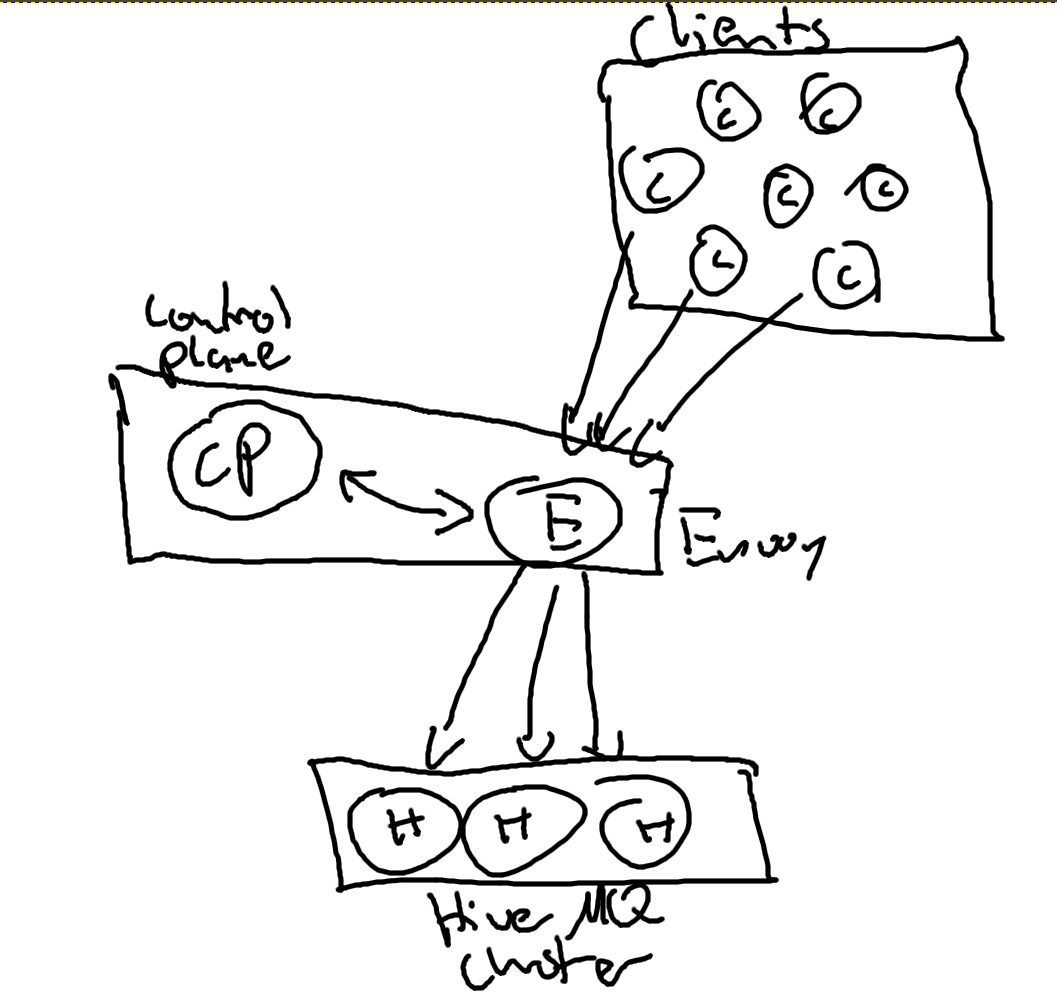
\includegraphics[scale=0.36]{images/control-plane-architecture.png}
    \caption{Die Abbildung zeigt die Architektur eines Envoy Load-Balancers konfiguriert von einer Control-Plane mit einem HiveMQ Cluster und MQTT Clients. Verbindungspfeile zwischen den einzelnen Komponenten sind Netzwerkverbindungen.}
    \label{fig:control-plane-architecture}
\end{figure}

\subsubsection{DNS Cluster-Discovery} \label{ss:dns-discovery}
Die Implementierung der HiveMQ Cluster-Discovery in der Control-Plane muss sich konzeptuell der \ac{dns} Cluster-Discovery von der HiveMQ Erweiterung anlehnen. Wie in Kapitel \ref{ss:cluster-discovery} beschrieben würde sonst die Topologie des HiveMQ Clusters im Envoy von der tatsächlichen Topologie divergieren.
\\
Die Control-Plane muss asynchron und periodisch einen gegebenen Domain-Namen auflösen und alle hinterlegten \ac{ip}-Adressen als Nodes eines HiveMQ Clusters eintragen. Das Intervall der periodischen Auflösung sollte sehr gering gehalten sein, um auf Topologieänderungen schnell reagieren zu können.
Cloudumgebungen wie Kubernetes haben in der Regel eigene \ac{dns} Services installiert, die eine hohe Abfragerate verarbeiten können.
\\
Quellcodeauszug \ref{code:dns-resolve-net} zeigt die Auflösung aller \ac{ip}-Adressen eines Domain-Namens in Golang mit der Standard \verb|net| Bibliothek.
Durch den Start der Funktion \verb|refreshDNS| als Go-Routine, wird in der \verb|main| Funktion ein Warten auf die Terminierung der \verb|refreshDNS| Funktion vermieden.
Die \verb|refreshDNS| Funktion erneuert die \ac{ip}-Adressen periodisch in gegebenem Intervall.
\begin{figure}
    \import{gen/}{dns-resolve-net}
    \caption{Der Quellcodeauszug zeigt die Auflösung aller \ac{ip} Adressen für einen gegebenen Domain-Namen in Golang.}
    \label{code:dns-resolve-net}
\end{figure}

\subsubsection{Weighted CPU Round-Robin} \label{ss:weighted-cpu}
Die Testszenarien aus Kapitel \ref{ss:test} zeigen, dass es bei \ac{mqtt} viele verschiedene Client-Verhaltensmuster gibt. Zudem kann ein Client sein Verhalten zur Laufzeit verändern.
Folglich kann der \acl{lb} diesen Client nicht mehr mit einem anderen Node verbinden.
Eine \ac{tcp}-Verbindung bei \ac{mqtt} korreliert nicht mit der verursachten Arbeitslast auf dem Broker. In Szenario zwei haben 300 Publisher doppelt so viel Last erzeugt wie 3.000 Subscriber und 1.000 Publisher zusammen.
Nur anhand der Anzahl aktiver Verbindungen pro Node kann im Fall \ac{mqtt} keine optimale load balancing Entscheidung getroffen werden.
\\
Über eine Control-Plane kann die Gewichtung einzelner Nodes eines Clusters im Envoy dynamisch angepasst werden.
Die Control-Plane muss periodisch und asynchron die aktuelle \ac{cpu} Auslastung eines jeden Nodes abfragen und darauf basierend die Nodes gewichten.
HiveMQ stellt die aktuelle \ac{cpu} Auslastung über die Prometheus Metriken zur Verfügung, die einen Wertebereich zwischen 0 und 100 hat. Dieser Wert ist über alle \ac{cpu} Kerne gemittelt.
Quellcodeauszug \ref{code:prometheus-curl} zeigt die Abfrage der Prometheus Metriken eines HiveMQ Brokers gefiltert nach \verb|cpu_total_total|. Der Datentyp dieser Metrik ist ein \textit{Gauge}, der einen einzelnen numerischen Wert darstellt.\cite{prometheusMetricTypesPrometheus} Der Wert beträgt in diesem Beispiel 5.0 und bedeutet, dass die aktuelle \ac{cpu} Auslastung über alle \ac{cpu} Kerne gemittelt fünf Prozent beträgt.
\begin{figure}
    \import{gen/}{prometheus-curl}
    \caption{Zeile 1 zeigt einen \textit{curl} Aufruf in einem Terminal, der Prometheus Metriken von einem lokalen HiveMQ Broker abfragt. Nachfolgend wird die Ausgabe mit einem \textit{grep} Befehl nach \textit{cpu\_total\_total} gefiltert. Zeile 3 bis 7 zeigen die Ausgabe im Terminal.}
    \label{code:prometheus-curl}
\end{figure}
\\
Für die programmatische Auswertung von Prometheus Metriken werden Bibliotheken für verschiedene Programmiersprachen bereitgestellt, so auch für Golang.
Das \verb|expfmt| Paket dieser Bibliothek ist für das Parsen der Metriken zuständig \cite{ExpfmtPkgGo}.
Quellcodeauszug \ref{code:expfmt} zeigt ein Golang Programm, das periodisch und asynchron die Prometheus Metrik \verb|com_hivemq_system_os_global_cpu_total_total| von einem HiveMQ Broker unter der Adresse \verb|http://localhost:9399/metrics| abruft. Der Wert der Metrik kann alle Werte zwischen 0 (keine Auslastung) und 100 (volle Auslastung) annehmen. Er wird in der Variable \verb|value| als Gleitkommazahl gespeichert.
\begin{figure}
    \import{gen/}{expfmt}
    \caption{Der Quellcodeauszug zeigt wie man in Golang Prometheus Metriken mit \textit{expfmt} und \textit{net/http} abfragen und parsen kann.}
    \label{code:expfmt}
\end{figure}
\\
Die \ac{cpu} Auslastung eines Nodes kann durch diverse Faktoren zeitweise schwanken. Mögliche Ursachen sind zum Beispiel der Java-Garbage-Collector, eine kurzfristige Traffic Spitze oder ein Client-Takeover.
Diese kurzfristigen Unterschiede der Auslastung dürfen nicht direkt zu einer Veränderung der Gewichtung des Nodes führen.
Um den direkten Einfluss solcher Spitzen zu vermeiden, werden Werte über einen bestimmten Zeitraum gesammelt und gemittelt. Der Mittelwert ist die durchschnittliche Arbeitslast eines Nodes in Prozent für eine bestimmte Dauer.
\\
Anschlie{\ss}end wird die durchschnittliche Arbeitslast in eine Gewichtung für Envoy konvertiert.
Je grö{\ss}er der Wert der Gewichtung im Vergleich zu den Gewichtungen der anderen Nodes ist, desto mehr Clients werden mit diesem Node verbunden (siehe Kapitel \ref{ss:weighted-rr}).
Demnach ist es nicht möglich, die durchschnittliche Arbeitslast direkt als Gewichtung zu benutzen. Es würde ein gegenteiliger Effekt entstehen.
\\
Da Nodes mit grö{\ss}eren Gewichtungen mehr Clients erhalten, wird die freie \ac{cpu} Auslastung als Gewichtung der Nodes gewählt.
Die freie Auslastung ergibt sich aus der Differenz von maximaler Auslastung (100) und durchschnittlicher Auslastung.
Wenn man die freie Auslastung als Gewichtung der Nodes wählt, verteilen sich neue Clients bei einem Cluster aus Tabelle \ref{table:example-cluster-cpu} wie folgt auf die Nodes:
\begin{itemize}
  \item \textbf{Node 1:}
    \begin{align}
      13 / (13 + 70 + 95 + 78) \cdot 100 \approx 5,1 \%
    \end{align}
  \item \textbf{Node 2:}
    \begin{align}
      70 / (13 + 70 + 95 + 78) \cdot 100 \approx 27,3 \%
    \end{align}
  \item \textbf{Node 3:}
    \begin{align}
      95 / (13 + 70 + 95 + 78) \cdot 100 \approx 37,1 \%
    \end{align}
  \item \textbf{Node 4:}
    \begin{align}
      78 / (13 + 70 + 95 + 78) \cdot 100 \approx 30,5 \%
    \end{align}
\end{itemize}
\begin{table}[h]
\centering
\renewcommand{\arraystretch}{1.5}
\begin{tabular}{|l|c|c|}
    \hline
    & \textbf{Ø CPU Auslastung} & \textbf{Ø freie CPU Kapazitäten} \\
    \hline
    \hline
    Node 1 & 87 \% & 13 \% \\
    \hline
    Node 2 & 30 \% & 70 \% \\
    \hline
    Node 3 & 5 \% & 95 \% \\
    \hline
    Node 4 & 22 \% & 78 \% \\
    \hline
\end{tabular}
\caption{CPU Auslastung und Kapazitäten von Nodes eines Clusters über einen beliebigen Zeitraum}
\label{table:example-cluster-cpu}
\end{table}
Nodes mit einer höheren Auslastung, zum Beispiel Node 1, erhalten nun weniger neue Clients als Nodes mit einer geringeren Auslastung wie Node 3.
\\
Um einen weighted \ac{cpu} round-robin \acl{lb} zu validieren, wurden ebenfalls die Testszenarien aus Kapitel \ref{ss:test} durchgeführt.
Tabelle \ref{table:test-output} zeigt die Standardabweichung der einzelnen Testszenarien verglichen mit einem round-robin und least-connection load balancing Algorithmus.
Nachdem sich alle \ac{mqtt} Clients aus den Testszenarien mit dem Cluster verbunden haben, wurden die Werte der Standardabweichung gemessen.
Abbildungen \ref{fig:s1-cpu}, \ref{fig:s2-cpu} und \ref{fig:s3-cpu} zeigen die zeitlichen Verläufe des weighted \ac{cpu} \aclp{lb} bei den Testszenarien eins, zwei und drei.
\\
Insgesamt erzielte der weighted round-robin load balancing Algorithmus die besten Ergebnisse.
Dieser weist eine leichte Optimierung gegenüber dem round-robin Algorithmus auf. Der least-connection Algorithmus hat die grö{\ss}te Standardabweichung der \ac{cpu} Auslastungen und bestätigt, dass \ac{mqtt} Verbindungen unterschiedliche Lastprofile aufweisen.
Die unterschiedlichen Lastverteilungen zwischen den load balancing Algorithmen kommen durch die unterschiedlichen Testszenarien zustande. Diese wurden basierend auf den Schwachstellen von round-robin und least-connection in Bezug auf \ac{mqtt} ausgelegt, um zu untersuchen, ob ein weighted round-robin load balancing Algorithmus basierend auf der \ac{cpu} Auslastung generell eine bessere Lastverteilung bietet.

\begin{table}[h!]
\centering
\renewcommand{\arraystretch}{1.5}
\begin{tabular}{|l|c|c|c|}
    \hline
    & round-robin & least-connection & weighted CPU \\
    \hline
    Testszenario 1 & 9 & 8 & 8 \\
    \hline
    Testszenario 2 & 3 & 10 & 4 \\
    \hline
    Testszenario 3 & 8 & 6 & 6 \\
    \hline
    \hline
    Gesamt & 20 & 24 & 18 \\
    \hline
\end{tabular}
\caption{Die Tabelle zeigt die Standardabweichungen der Testszenarien aus Kapitel \ref{ss:test} und des weighted round-robin load balancing Algorithmus.}
\label{table:test-output}
\end{table}

% TODO center images
\begin{figure}[h!]
    \centering
    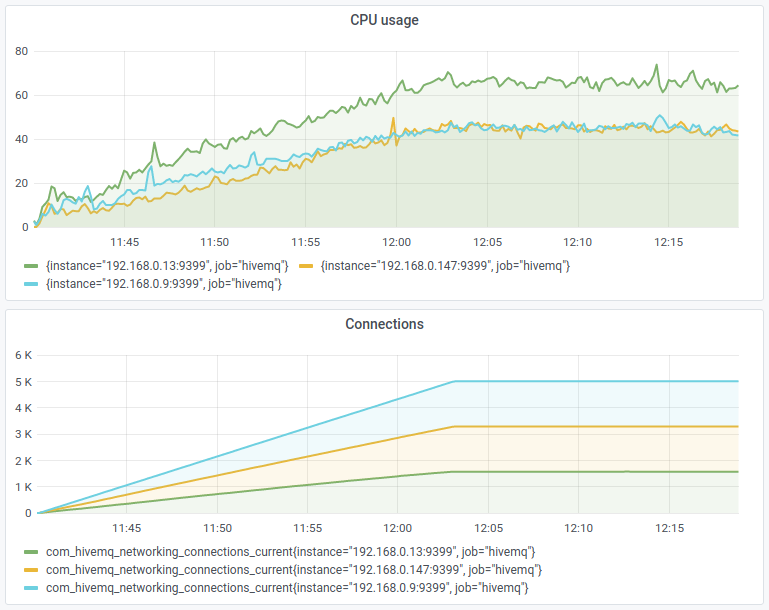
\includegraphics[scale=0.8]{images/s1_cpu.png}
    \caption{Testszenario 1 - weighted CPU round-robin \acl{lb}}
    \label{fig:s1-cpu}
\end{figure}

\begin{figure}[h!]
    \centering
    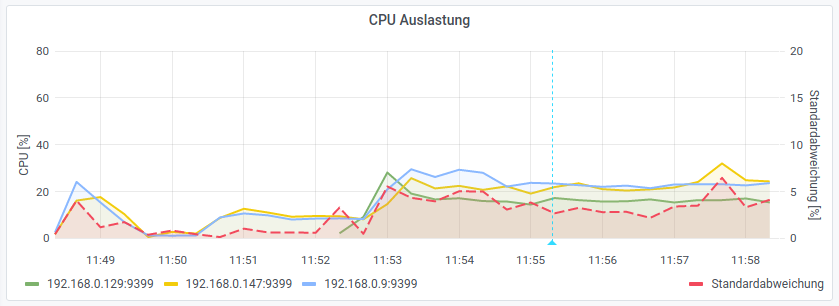
\includegraphics[scale=0.8]{images/s2_cpu.png}
    \caption{Testszenario 2 - weighted CPU round-robin \acl{lb}}
    \label{fig:s2-cpu}
\end{figure}

\begin{figure}[h!]
    \centering
    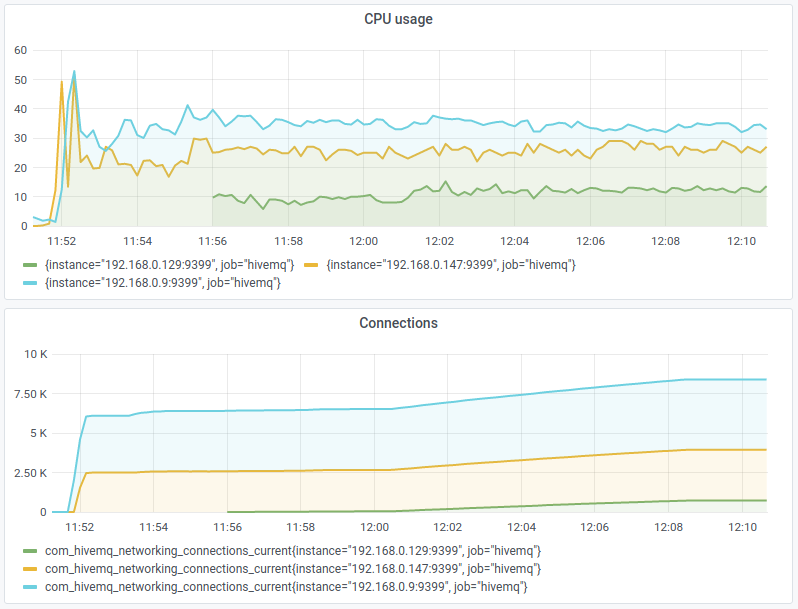
\includegraphics[scale=0.8]{images/s3_cpu.png}
    \caption{Testszenario 3 - weighted CPU round-robin \acl{lb}}
    \label{fig:s3-cpu}
\end{figure}

\newpage
\null
\newpage
\subsubsection{Überlastschutz} \label{ss:circuit-breaking}
Wie in Kapitel \ref{ss:weighted-cpu} beschrieben, kann das Lastverhalten von \ac{mqtt} Clients während der Laufzeit stark variieren.
Da ein Client zur Laufzeit nicht mit einem anderen Node verbunden werden kann, führt es bei dem Verändern des Lastverhaltens von Clients zu einer Überlastsituation eines Nodes.
Ein HiveMQ Broker hat mehrere Möglichkeiten, sich vor einer solchen Überlastsituation zu schützen (siehe Kapitel \ref{sb:overload-protection}).
Im ersten Schritt wendet der Broker \ac{tcp} \textit{Back pressure} auf individuelle Clientverbindungen an, um den Paketfluss zu verzögern.
Führt diese Mechanik nicht zur gewünschten Kontrolle der Lastspitze, wird die Verbindung zu allen Clients unterbrochen, die ihre Credits aufgebraucht haben.
Dadurch werden gezielt Clients vom Broker getrennt, die zu viel Arbeitslast für den Broker verursachen.
Durch die Trennung dieser Clients gibt es keine Serviceeinschränkungen für alle anderen Clients, die mit dem Broker verbunden sind.
Sonst käme es zu Paketverzögerungen oder Paketverlusten auf einem Broker.
\\
Wenn sich ein Node eines Clusters in einer Überlastsituation befindet, ist es wichtig, dass der \acl{lb} keine neuen Clients mehr mit diesem Node verbindet.
Über die Prometheus Schnittstelle der HiveMQ Nodes werden diverse Metriken über den Zustand eines Nodes abgefragt.
Eine Liste aller Prometheus Metriken findet sich in der HiveMQ Dokumentation \cite{MonitoringHiveMQDocumentation}.
Tabelle \ref{table:overload-protection-metrics} gibt eine Übersicht der Metriken, die Indikatoren für eine mögliche Überlastsituation sind. Metriken, die sich auf Clients beziehen, enthalten nur Daten von Clients, die mit dem Node verbunden sind und bei dem die Metriken abgefragt wurden.
\begin{table}[htbp]
\centering
\renewcommand{\arraystretch}{1.5}
\begin{tabularx}{\textwidth}{|p{5cm}|X|}
    \hline
    \textbf{Metrik} & \textbf{Beschreibung} \\
    \hline
    \hline
    \verb|com.hivemq.supervision.| \verb|overload.protection.level| & Aktueller \textit{Overload-Protection Level} zwischen 1 und 10. \\
    \hline
    \verb|com.hivemq.overload-| \verb|protection.credits.| \verb|per-tick| & Anzahl der Credits, die ein Client alle 200 Millisekunden regeneriert. \\
    \hline
    \verb|com.hivemq.overload-| \verb|protection.clients.| \verb|average-credits| & Durchschnittliche Anzahl der Credits aller Clients. \\
    \hline
    \verb|com.hivemq.overload-| \verb|protection.clients.| \verb|backpressure-active| & Anzahl der Clients, die durch eine Overload-Protection \ac{tcp} Back pressure haben. \\
    \hline
\end{tabularx}
\caption{Die Tabelle zeigt HiveMQ Metriken, die in einer Beziehung zu dem Overload-Protection Level stehen.}
\label{table:overload-protection-metrics}
\end{table}
\\
Die Metrik \verb|com.hivemq.supervision.overload.protection.level| aggregiert intern \newline mehrere Metriken zusammen und bestimmt einen allgemeinen Überlastlevel des Nodes.
Der Wert des Levels liegt zwischen null und maximal zehn.
Um ein maximales Überlastlevel zu vermeiden, kann der \acl{lb} präventiv keine neuen Clients mehr mit einem Node verbinden, der einen bestimmten Schwellwert als Level überschritten hat.
\\
Ein hohes Überlastlevel kann kurzfristig durch Events wie das Beitreten eines neuen Nodes in ein Cluster auftreten. Dabei werden einige Client-Queues auf den neuen Node repliziert, was zeitweise die Nodes, auf denen die Queues liegen, stark beansprucht. Es ist wichtig, dass der \ac{lb} auf solche Events schnell reagiert und keine neuen Clients mehr mit den betroffenen Nodes verbindet.
Um dies zu gewährleisten, wird eine geringe Abtastfrequenz der Prometheus Metriken gewählt.
\\
Eine in Abbildung \ref{fig:overload-protection} gezeigte Überlastsituation verursacht einen maximalen Überlastlevel von zehn. Dieser wird zu Beginn durch das Beitreten eines dritten Nodes und einem Verbinden von 800 Clients ausgelöst.
Um ein HiveMQ Cluster in dieser Situation zu unterstützen, kann ein Schwellenwert für den Überlastschutz auf vier gesetzt werden, damit sich keine neuen Clients mehr mit einem in Überlastsituation befindenden Node verbinden.
In Kombination mit der Möglichkeit, \ac{tcp} Back pressure bei Clients anzuwenden, kann HiveMQ eine solche Überlastsituation kontrollieren, ohne die Verbindungen der Clients zu unterbrechen.
Diese Methode wird auch als \textit{load-shedding} bezeichnet.
Dabei reduziert sich der angebotene Service für einige Clients, um das Gesamtsystem aufrechtzuerhalten.
\\
\begin{figure}
    \centering
    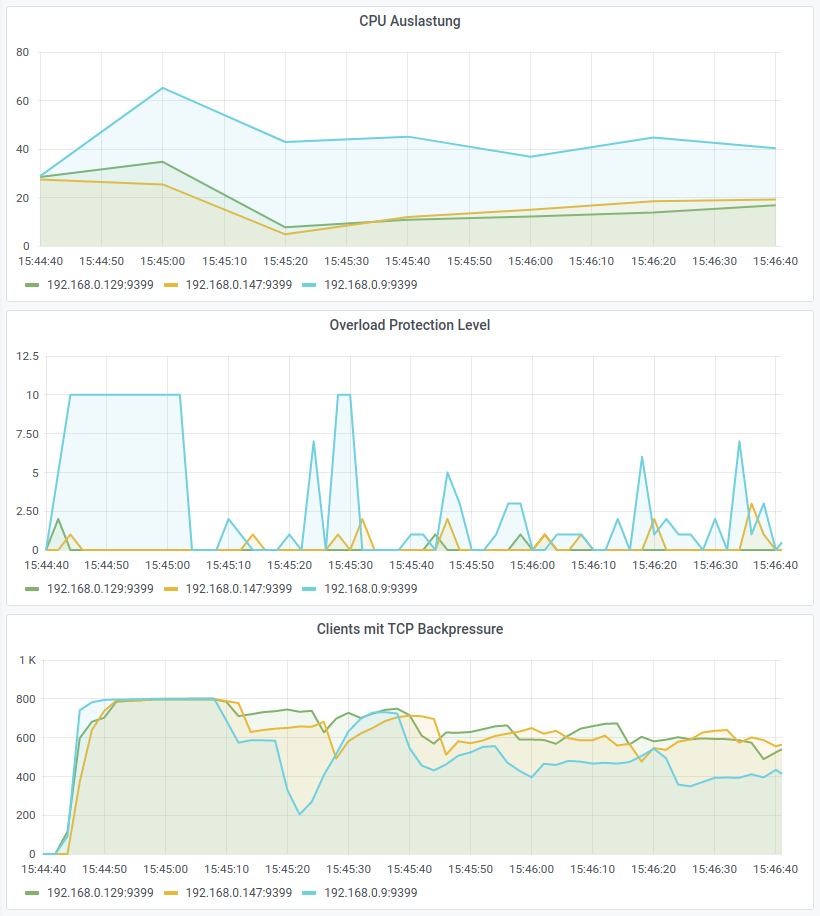
\includegraphics[scale=0.8]{images/overload-protection.png}
    \caption{Die Abbildung zeigt Prometheus Metriken, die mit Grafana dargestellt werden, von einem HiveMQ Cluster bestehend aus drei Nodes. Bei den \ac{mqtt} Clients, die mit dem Cluster verbunden sind, wird von dem Broker \ac{tcp} backpressure angewendet, da diese zu viele Nachrichten veröffentlichen.}
    \label{fig:overload-protection}
\end{figure}
Um Envoy zu instruieren, keine neuen Clients mit einem sich in einer Überlastsituation befindenden HiveMQ Node zu verbinden, wird der \textit{Health-Status} des Nodes entsprechend gesetzt.
Der Wert ist entweder \verb|HEALTHY| oder \verb|UNHEALTHY|.
Dieser Zustand kann über die Control-Plane für jeden Node individuell gesetzt werden.
\cite{HealthCheckEnvoy}
Die Funktionalität des Health-Status eines Nodes wird in Kapitel \ref{ss:health-check} detailliert betrachtet.
\newpage

\subsubsection{Health-Check} \label{ss:health-check}
Nodes eines Clusters in Envoy haben einen Gesundheitszustand (engl. \textit{Health-Status}) der angibt, ob ein Node neue Clientverbindungen erhalten kann.
Der Health-Status eines Nodes ist anwendungsspezifisch und kann unter anderem durch \textit{health-checks} bestimmt werden.
\ac{http}-Services implementieren für diesen Zweck beispielsweise eine \verb|/health| Route, die der \acl{lb} periodisch abrufen kann. Wenn der \ac{http}-Status-Code der Antwort 200 beträgt, ist der Service \textit{healthy} und bereit für neue Verbindungen.
\\
Um zu überprüfen, ob ein HiveMQ Broker bereit ist, neue Clientverbindungen \ac{mqtt} konform anzunehmen, muss sich die Control-Plane als \ac{mqtt} Client bei dem Broker anmelden.
Bei einer erfolgreichen Verbindung wird die \ac{mqtt} Verbindung \ac{mqtt} konform beendet und der Node als \verb|HEALTHY| markiert.
Um einen ausführlicheren Health-Check zu implementieren, können noch weitere \ac{mqtt} Funktionen wie Publish und Subscribe getestet werden. Dazu abonniert die Control-Plane ein Topic, das nicht von anderen Clients verwendet wird. Nach dem Abonnieren veröffentlicht die Control-Plane eine beliebige Nachricht auf dem zuvor abonnierten Topic und überprüft, ob diese Nachricht empfangen wird. Abbildung \ref{fig:health-check-sequence} zeigt die erforderlichen \ac{mqtt} Pakete und den Ablauf des beschriebenen Health-Checks in einem UML Ablaufdiagramm. Wenn keine Fehler während des Health-Checks auftreten, wird der Node als \verb|HEALTHY| markiert.
\\
Um Clients möglichst immer mit einem funktionierenden HiveMQ Node eines Clusters zu verbinden, muss der Health-Check periodisch von der Control-Plane ausgeführt werden.
Zudem kann ein Zeitfenster definiert werden, in dem ein Health-Check erfolgreich durchgelaufen sein muss.
Falls der Health-Check länger als das Zeitfenster benötigt, gilt der Node als \verb|UNHEALTHY|.
Dadurch wird neben der Funktionalität des Brokers auch eine gegebene Antwortzeit gewährleistet.
\begin{figure}
    \centering
    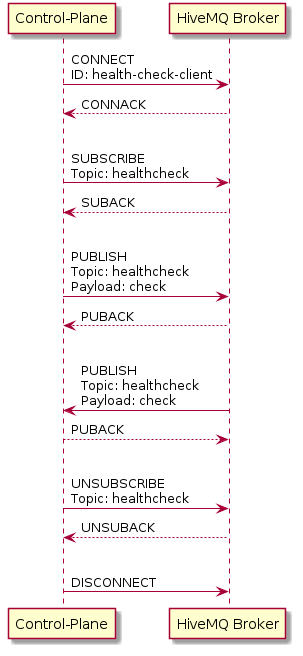
\includegraphics[scale=0.6]{gen/health-check.png}
    \caption{Die Grafik zeigt ein UML Ablaufdiagramm des in Kapitel \ref{ss:health-check} erläuterten \ac{mqtt} Health-Checks.}
    \label{fig:health-check-sequence}
\end{figure}

\newpage
\subsubsection{Aktualisierung der Konfiguration}
Um Aktualisierungen wie Health-Status, Gewichtung oder Anzahl der Nodes an eine Envoy Instanz zu schicken, werden versionierte Momentaufnahmen (engl. \textit{Snapshots}) von einem Zustand der Konfiguration erstellt. Wenn die Version des Snapshots auf dem Envoy eine andere Version ist als die Version des aktuellen Snapshots auf der Control-Plane, liefert die Control-Plane den aktuellen Snapshot an die Envoy Instanz aus.
\\
Um Konfigurationen optimal in einem Cache-Speicher abzulegen, hat eine einzigartige Konfiguration immer dieselbe Version.
Dazu kann die Clusterkonfiguration in eine Hash-Funktion gegeben werden, um als Resultat einen String mit fixer Länge als Rückgabewert zu erhalten.
Die Hash-Funktion garantiert einen immer gleichen Rückgabewert bei gleichem Input. Dementsprechend wird bei gleichbleibender Konfiguration immer die gleiche Version erzeugt.
Als Eingabe der Hash-Funktion dienen alle Informationen, bei deren Änderung eine neue Version erstellt werden soll. Dies ist eine Liste aller HiveMQ Nodes mit folgenden Werten:
\begin{itemize}
  \item \ac{ip}-Adresse
  \item Port
  \item Gewichtung
  \item Health-Status
\end{itemize}
Die Reihenfolge, in der die Nodes in der Liste für die Hash-Funktion vorkommen, ist von hoher Relevanz.
Hätten alle Nodes dieselben Werte, sich aber die Reihenfolge der Liste ändert, würde die Hash-Funktion einen neuen Wert zurückgeben.
Daher muss sichergestellt sein, dass die Nodes immer in der gleichen Reihenfolge vorkommen.
Um die Liste der Nodes zu sortieren, werden einzigartige Eigenschaften der Nodes verglichen.
Es können niemals zwei HiveMQ Nodes dieselbe \ac{ip}-Adresse und denselben Port haben. Beide Werte als String vereint können verglichen werden, um bei gleichbleibenden Nodes dieselbe Reihenfolge in einer Liste einzuhalten.
\begin{figure}
    \import{gen/}{snapshot-versioning}
    \caption{Der Quellcodeauszug zeigt die Generierung einer Envoy Snapshot Version basierend der HiveMQ Node Eigenschaften Hostname, Port, Gewichtung und Health-Status in Golang.}
    \label{code:snapshot-versioning}
\end{figure}
\\
Die Funktion \verb|generateVersion| aus Quellcodeauszug \ref{code:snapshot-versioning} generiert die Version für einen Snapshot. Es wird eine HiveMQ Node Liste übergeben und ein String zurückgegeben, der als Version des Snapshots dient. Nach der Sortierung der HiveMQ Node Liste nach Identifier, der aus Hostnamen und Port besteht, werden die Werte Identifier, Gewichtung und Health-Status in eine Hash-Funktion gegeben. Das Ergebnis der Hash-Funktion ist der Rückgabewert der Funktion \verb|generateVersion|.
\newpage

\subsection{Sticky Session} \label{ss:sticky-session}
Ein HiveMQ Broker speichert temporär Daten von \ac{mqtt} Clients ab.
Darunter sind Daten wie zum Beispiel Topic Aliasse oder Nachrichten, die aufgrund eines Verbindungsabbruchs nicht zugestellt werden konnten.
Sobald sich ein nicht mehr verbundener Client wieder mit dem Broker verbindet, kann der Broker die vorbehaltenen Nachrichten zustellen.
Dies verringert den Datenverlust in instabilen Netzwerken.
\\
Wie in Kapitel \ref{sp:persistent-session} erläutert, werden clientspezifische Daten nur auf bestimmten HiveMQ Nodes eines Clusters gespeichert.
Wenn die Verbindung eines Clients unterbrochen wird und beim Verbindungsaufbau mit einem anderen Node als zuvor verbunden wird, müssen die Daten des Clients im Cluster synchronisiert werden.
Im Optimalfall verbindet sich der Client mit demselben Node wie zuvor, wodurch keine Synchronisation notwendig ist.
Ein solches Verfahren nennt sich \textit{Sticky-Session} oder \textit{Session-Affinity}. Dabei werden einzigartige Identifier eines Clients im \acl{lb} extrahiert, und beispielsweise in einer HashMap mit dem Zielnode gespeichert. Sobald der Client eine erneute Verbindung aufbaut, kann der \acl{lb} in der HashMap den alten Node nachschlagen und den Client mit diesem Node verbinden. \cite{WhatDoesTerm}

\subsubsection{Clientkennung} \label{ss:clientid}
Jeder \ac{mqtt} Client identifiziert sich durch eine einzigartige Clientkennung. Dieser wird, wie in Kapitel \ref{s:mqtt-connect} beschrieben, in dem \ac{mqtt} \verb|CONNECT| Paket beim Verbindungsaufbau vom Client an den Broker geschickt.
Eine Clientkennung darf niemals doppelt vergeben werden. Sobald sich ein Client mit dem Broker verbindet, dessen Kennung bereits von einem anderen Client genutzt wird, unterbricht der Broker die Verbindung mit dem bereits verbundenen Client und führt einen Client-Takeover durch.
Dieser Vorgang gewährleistet, dass jede Clientkennung nur einmal vergeben ist.
\\
Die Clientkennung eignet sich durch ihre Einzigartigkeit als Identifier für eine Sticky-Session.

\subsubsection{MQTT CONNECT}
In Kapitel \ref{ss:clientid} wurde die Benutzung der \ac{mqtt} Clientkennung als Merkmal für eine Sticky Session beschrieben. Envoy ist im Kern ein \ac{osi}-Layer vier Proxy und hat auf Informationen, wie eine Layer sieben \ac{mqtt} Clientkennung, keinen Zugriff. Wie in Kapitel \ref{s:envoy} erläutert, kann Envoy zum Beispiel für \ac{http} als Layer sieben \ac{lb} betrieben werden, da das Dekodieren von \ac{http}-Paketen bereits in Envoy implementiert wurde.
Das \ac{mqtt} Protokoll ist nicht in Envoy integriert. Aus diesem Grund gibt es keine Möglichkeit in der Envoy Konfiguration eine load balancing Entscheidung anhand der Clientkennung zu treffen, da Envoy die einzelnen \ac{mqtt} Pakete nicht dekodiert.
\\
Envoy ermöglicht das Einbinden von \acl{wasm}-Modulen als Netzwerkfilter.
Ein Netzwerkfilter könnte \ac{mqtt} Pakete dekodieren, um diese den nachfolgenden Filtern in der Pipeline zur Verfügung zu stellen.
Bislang gibt es \ac{wasm} \acp{sdk} für Rust, C++, AssemblyScript und Golang. \cite{sebastianHowWriteWASM} Beispiele für eine Implementation eines Golang Netzwerk Filters finden sich auf GitHub \cite{TetratelabsProxywasmgosdk2021}.
\\
Das Dekodieren der \ac{mqtt} Pakete in Golang wurde bereits von der Eclipse \ac{mqtt} Bibliothek \cite{EclipsePahoMqtt2021} implementiert.
Der Quellcodeauszug \ref{code:mqtt-connect-decode} zeigt einen Auszug aus der Datei \verb|packets/connect.go| des Repositories und dekodiert ein \ac{mqtt} \verb|CONNECT| Paket. Die Fehlerabhandlung wurde für eine bessere Lesbarkeit entfernt. Quellcodeauszug \ref{code:mqtt-connect-struct} zeigt die Struktur eines \verb|CONNECT| Paketes basierend auf den in Kapiel \ref{s:mqtt-connect} beschriebenen Feldern.
\begin{figure}[h]
    \import{gen/}{mqtt-connect-struct}
    \caption{Es wird eine Golang Struktur gezeigt, die alle Daten eines \ac{mqtt} CONNECT Paketes beinhalten kann. Quelle: \cite{EclipsePahoMqtt2021}}
    \label{code:mqtt-connect-struct}
\end{figure}
\begin{figure}[h]
    \import{gen/}{mqtt-connect-decode}
    \caption{Der Quellcodeauszug zeigt eine Golang Funktion, die ein \ac{mqtt} CONNECT Paket dekodiert. Quelle: \cite{EclipsePahoMqtt2021}}
    \label{code:mqtt-connect-decode}
\end{figure}
\\
Bei jeder neuen Clientverbindung dekodiert der \acl{lb} das erste Paket des Clients mit der Funktion \verb|Unpack| aus Quellcodeauszug \ref{code:mqtt-connect-decode}, um an den Wert von\newline
\verb|ConnectPacket.ClientIdentifier| zu gelangen.
Die Clientkennung wird beispielsweise in einer HashMap gespeichert, um bei neuen Clientverbindungen zu prüfen, ob der Client bereits mit einem Node verbunden wurde.

\newpage
\subsubsection{Cluster Health}
Bei dem in Kapitel \ref{ss:weighted-cpu} vorgestellten weighted round-robin load balancing Algorithmus ist es nicht möglich, einen individuellen Client mit einem bestimmten Node zu verbinden.
Der \acl{lb} entscheidet, ob ein Client basierend auf dem weighted round-robin oder dem Sticky-Session Algorithmus aus Kapitel \ref{ss:clientid} mit einem Zielnode verbunden wird.
\\
Eine Möglichkeit, beide Algorithmen in einem \acl{lb} zu verwenden, ist bei einem neuen Client zuerst in der HashMap nachzuschlagen, ob dieser Client bereits mit einem Node verbunden wurde. Falls dieser Node noch vorhanden und \verb|HEALTHY| ist, wird der Client erneut mit dem Node verbunden. Andernfalls wird ein neuer Node basierend dem weighted round-robin Algorithmus bestimmt.
Diese Methode harmoniert mit dem beschriebenen Überlastschutz aus Kapitel \ref{ss:circuit-breaking}. Für den Fall, dass ein HiveMQ Node die Verbindung eines Clients aufgrund einer Überlastung unterbricht, markiert der Überlastschutz diesen Node als \verb|UNHEALTHY| und der \acl{lb} wird den Client, der sich wieder mit dem Cluster verbindet, mit einem anderen Node verbinden.
\\
Durch diese Implementation der Sticky Session werden Clients, die ihre Verbindung verlieren, immer mit demselben Node verbunden und Clients, deren Verbindung absichtlich beendet wurde, werden einem neuen Node zugewiesen. Clients, die sich zum ersten Mal mit dem Cluster verbinden, werden basierend auf der freien Arbeitslast verteilt.
\newpage
